\documentclass{article}

  % packages
    % basic stuff for rendering math
    \usepackage[letterpaper, top=1in, bottom=1in, left=1in, right=1in]{geometry}
    \usepackage[utf8]{inputenc}
    \usepackage[english]{babel}
    \usepackage{amsmath} 
    \usepackage{amssymb}

    % extra math symbols and utilities
    \usepackage{mathtools}        % for extra stuff like \coloneqq
    \usepackage{mathrsfs}         % for extra stuff like \mathsrc{}
    \usepackage{centernot}        % for the centernot arrow 
    \usepackage{bm}               % for better boldsymbol/mathbf 
    \usepackage{enumitem}         % better control over enumerate, itemize
    \usepackage{hyperref}         % for hypertext linking
    \usepackage{xr-hyper}
    \usepackage{fancyvrb}          % for better verbatim environments
    \usepackage{newverbs}         % for texttt{}
    \usepackage{xcolor}           % for colored text 
    \usepackage{listings}         % to include code
    \usepackage{lstautogobble}    % helper package for code
    \usepackage{parcolumns}       % for side by side columns for two column code
    

    % page layout
    \usepackage{fancyhdr}         % for headers and footers 
    \usepackage{lastpage}         % to include last page number in footer 
    \usepackage{parskip}          % for no indentation and space between paragraphs    
    \usepackage[T1]{fontenc}      % to include \textbackslash
    \usepackage{footnote}
    \usepackage{etoolbox}

    % for custom environments
    \usepackage{tcolorbox}        % for better colored boxes in custom environments
    \tcbuselibrary{breakable}     % to allow tcolorboxes to break across pages

    % figures
    \usepackage{pgfplots}
    \pgfplotsset{compat=1.18}
    \usepackage{float}            % for [H] figure placement
    \usepackage{tikz}
    \usepackage{tikz-cd}
    \usepackage{circuitikz}
    \usetikzlibrary{arrows}
    \usetikzlibrary{positioning}
    \usetikzlibrary{calc}
    \usepackage{graphicx}
    \usepackage{algorithmic}
    \usepackage{caption} 
    \usepackage{subcaption}
    \captionsetup{font=small}

    % for tabular stuff 
    \usepackage{dcolumn}

    \usepackage[nottoc]{tocbibind}
    \pdfsuppresswarningpagegroup=1
    \hfuzz=5.002pt                % ignore overfull hbox badness warnings below this limit

  % New and replaced operators
    \DeclareMathOperator{\Tr}{Tr}
    \DeclareMathOperator{\Sym}{Sym}
    \DeclareMathOperator{\Span}{span}
    \DeclareMathOperator{\std}{std}
    \DeclareMathOperator{\Cov}{Cov}
    \DeclareMathOperator{\Var}{Var}
    \DeclareMathOperator{\Corr}{Corr}
    \DeclareMathOperator{\pos}{pos}
    \DeclareMathOperator*{\argmin}{\arg\!\min}
    \DeclareMathOperator*{\argmax}{\arg\!\max}
    \newcommand{\ket}[1]{\ensuremath{\left|#1\right\rangle}}
    \newcommand{\bra}[1]{\ensuremath{\left\langle#1\right|}}
    \newcommand{\braket}[2]{\langle #1 | #2 \rangle}
    \newcommand{\qed}{\hfill$\blacksquare$}     % I like QED squares to be black

  % Custom Environments
    \newtcolorbox[auto counter, number within=section]{question}[1][]
    {
      colframe = orange!25,
      colback  = orange!10,
      coltitle = orange!20!black,  
      breakable, 
      title = \textbf{Question \thetcbcounter ~(#1)}
    }

    \newtcolorbox[auto counter, number within=section]{exercise}[1][]
    {
      colframe = teal!25,
      colback  = teal!10,
      coltitle = teal!20!black,  
      breakable, 
      title = \textbf{Exercise \thetcbcounter ~(#1)}
    }
    \newtcolorbox[auto counter, number within=section]{solution}[1][]
    {
      colframe = violet!25,
      colback  = violet!10,
      coltitle = violet!20!black,  
      breakable, 
      title = \textbf{Solution \thetcbcounter}
    }
    \newtcolorbox[auto counter, number within=section]{lemma}[1][]
    {
      colframe = red!25,
      colback  = red!10,
      coltitle = red!20!black,  
      breakable, 
      title = \textbf{Lemma \thetcbcounter ~(#1)}
    }
    \newtcolorbox[auto counter, number within=section]{theorem}[1][]
    {
      colframe = red!25,
      colback  = red!10,
      coltitle = red!20!black,  
      breakable, 
      title = \textbf{Theorem \thetcbcounter ~(#1)}
    } 
    \newtcolorbox[auto counter, number within=section]{proposition}[1][]
    {
      colframe = red!25,
      colback  = red!10,
      coltitle = red!20!black,  
      breakable, 
      title = \textbf{Proposition \thetcbcounter ~(#1)}
    } 
    \newtcolorbox[auto counter, number within=section]{corollary}[1][]
    {
      colframe = red!25,
      colback  = red!10,
      coltitle = red!20!black,  
      breakable, 
      title = \textbf{Corollary \thetcbcounter ~(#1)}
    } 
    \newtcolorbox[auto counter, number within=section]{proof}[1][]
    {
      colframe = orange!25,
      colback  = orange!10,
      coltitle = orange!20!black,  
      breakable, 
      title = \textbf{Proof. }
    } 
    \newtcolorbox[auto counter, number within=section]{definition}[1][]
    {
      colframe = yellow!25,
      colback  = yellow!10,
      coltitle = yellow!20!black,  
      breakable, 
      title = \textbf{Definition \thetcbcounter ~(#1)}
    } 
    \newtcolorbox[auto counter, number within=section]{example}[1][]
    {
      colframe = blue!25,
      colback  = blue!10,
      coltitle = blue!20!black,  
      breakable, 
      title = \textbf{Example \thetcbcounter ~(#1)}
    } 
    \newtcolorbox[auto counter, number within=section]{code}[1][]
    {
      colframe = green!25,
      colback  = green!10,
      coltitle = green!20!black,  
      breakable, 
      title = \textbf{Code \thetcbcounter ~(#1)}
    } 
    \newtcolorbox[auto counter, number within=section]{algo}[1][]
    {
      colframe = green!25,
      colback  = green!10,
      coltitle = green!20!black,  
      breakable, 
      title = \textbf{Algorithm \thetcbcounter ~(#1)}
    } 

    \definecolor{dkgreen}{rgb}{0,0.6,0}
    \definecolor{gray}{rgb}{0.5,0.5,0.5}
    \definecolor{mauve}{rgb}{0.58,0,0.82}
    \definecolor{darkblue}{rgb}{0,0,139}
    \definecolor{lightgray}{gray}{0.93}
    \renewcommand{\algorithmiccomment}[1]{\hfill$\triangleright$\textcolor{blue}{#1}}

    % default options for listings (for code)
    \lstset{
      autogobble,
      frame=ltbr,
      language=Python,
      aboveskip=3mm,
      belowskip=3mm,
      showstringspaces=false,
      columns=fullflexible,
      keepspaces=true,
      basicstyle={\small\ttfamily},
      numbers=left,
      firstnumber=1,                        % start line number at 1
      numberstyle=\tiny\color{gray},
      keywordstyle=\color{blue},
      commentstyle=\color{dkgreen},
      stringstyle=\color{mauve},
      backgroundcolor=\color{lightgray}, 
      breaklines=true,                      % break lines
      breakatwhitespace=true,
      tabsize=3, 
      xleftmargin=2em, 
      framexleftmargin=1.5em, 
      stepnumber=1
    }

  % Page style
    \pagestyle{fancy}
    \fancyhead[L]{Other Models}
    \fancyhead[C]{Muchang Bahng}
    \fancyhead[R]{Spring 2025} 
    \fancyfoot[C]{\thepage / \pageref{LastPage}}
    \renewcommand{\footrulewidth}{0.4pt}          % the footer line should be 0.4pt wide
    \renewcommand{\thispagestyle}[1]{}  % needed to include headers in title page

  % external documents 
  %  \externaldocument[place-]{../Machine_Learning/paper}[../Machine_Learning/paper.pdf] 

\begin{document}

\title{Other Models}
\author{Muchang Bahng}
\date{Spring 2025}

\maketitle
\tableofcontents
\pagebreak

This covers computability theory, complexity theory, and automata theory. 
Alphabet. Boolean logic


\section{Topological Data Analysis}

\section{Geodesic Regression}

  In regression, note that we are finding a function $f: \mathcal{X} \to \mathcal{Y}$. In usual linear regression, both $\mathcal{X}, \mathcal{Y}$ are Euclidean space. However, there are cases where it may not be realistic that one or more of them should be modeled as a vector space. Rather, they may be part of a lower-dimensional manifold. For instance, if we want to use linear regression to predict the top $k$ principal components of a dataset, they must be orthogonal, i.e. must be in a \textit{Stiefl manifold}. 

  There are way to model this. For instance, we could have a projection operator that maps from $\mathbb{R}^m \to \mathcal{Y}$. This has its issues too, for one not being very efficient since perhaps the dimension of $\mathcal{Y}$ may be much less than $m$. Therefore, it might be better to directly regress onto a manifold. There were many attempts at this, but the first model to generalize OLS to manifolds was created by Fletcher in 2011 \cite{2011fletcher} and expanded shortly in \cite{2012fletcher}. 

  We start with the case where there is one covariate (i.e. $\mathcal{X} = \mathbb{R}$) and $\mathcal{Y} = (M, d)$ is a smooth Riemannian manifold with a metric. Recall that for a smooth manifold $M$, for any $p \in M$ and $v \in T_p M$, the tangent space at $p$, there is a unique geodesic curve $\gamma: [0, 1] \to M$ satisfying $\gamma(0) = p$, $\gamma^\prime (0) = v$. This geodesic is guaranteed to exist locally, and with this,we can define the exponential map at $p$ in the direction of $v$ as 
  \begin{equation}
    \exp_p (v) = \exp(p, v) = \gamma(1)
  \end{equation}
  In other words, the exponential map takes a position and velocity as input and returns the point at time 1 along the geodesic with these initial conditions. With this motivation, we use slightly different notation than regular linear regression, referring $p$ as the bias and $v$ as the coefficient. 

  \begin{definition}[Geodesic Regression] 
    The \textbf{geodesic regression} model is a probabilistic model that predicts the conditional distribution of $y \in (M, d)$ given $x \in \mathbb{R}$ as 
    \begin{equation}
      y = \exp(\exp(p, vx), \epsilon)
    \end{equation} 
    where the parameters are $\theta = \{p, v\}$, and $\epsilon$ is a random variable defined over the tangent space at $\exp(p, vx)$. 
  \end{definition} 

  Note that if we set $\mathcal{Y} = \mathbb{R}^m$, then we get the ordinary linear regression model back. 

  \begin{definition}[Least Squares Geodesic Regression]
    The least squares geodesic regression aims to minimize the MSE loss 
    \begin{equation}
      L(\theta, (x, y)) = L(p, v, x, y) = d(\exp(p, vx), y)^2
    \end{equation}
  \end{definition}

  \begin{lemma}[Risk]
    The risk is 
    \begin{equation}
      R(f) = \mathbb{E}_{x, y} \left[ d(\exp(p, vx), y)^2 \right]
    \end{equation} 
    and the empirical risk for a dataset $\mathcal{D} = \{(x^{(i)}, y^{(i)})\}_{i=1}^n$ is 
    \begin{equation}
      \hat{R}(f) = \frac{1}{n} \sum_{i=1}^n d(\exp(p, v x^{(i)}), y^{(i)})^2
    \end{equation}
  \end{lemma}

  Unfortunately, minimizing this does not yield an analytic solution. 

  \begin{example}[Code Walkthrough]
    Let us fit a line onto this. We first define our manifold class with the matrix exponential and logarithm methods. 

    \begin{lstlisting}
      class S2:
        @staticmethod
        def exp(p, v):
          v_norm = np.linalg.norm(v)
          if v_norm < 1e-8:
            return p
          return np.cos(v_norm) * p + np.sin(v_norm) * v / v_norm
        
        @staticmethod
        def log(p, q):
          cos_dist = np.clip(np.dot(p, q), -1, 1)
          if np.abs(cos_dist - 1) < 1e-8:
            return np.zeros_like(p)
          
          theta = np.arccos(cos_dist)
          sin_theta = np.sin(theta)
          
          if sin_theta < 1e-8:
            return np.zeros_like(p)
          
          return theta * (q - cos_dist * p) / sin_theta
        
        @staticmethod
        def distance(p, q):
          cos_dist = np.clip(np.dot(p, q), -1, 1)
          return np.arccos(cos_dist)
        
        @staticmethod
        def project_to_tangent(p, v):
          return v - np.dot(v, p) * p
        
        @staticmethod
        def normalize(x):
          return x / np.linalg.norm(x)
    \end{lstlisting}

    Next, we define our data generation process. 

    \begin{lstlisting}
      def generate_sample_data(n_samples=50, noise_level=0.1):
        X = np.random.uniform(-2, 2, n_samples)
        
        p_true = S2.normalize(np.array([1, 0, 0]))
        v_true = S2.normalize(np.array([0, 1, 0.2]))
        v_true = S2.project_to_tangent(p_true, v_true) * 0.5
        
        Y = []
        for x in X:
          y_clean = S2.exp(p_true, v_true * x)
          
          noise = np.random.normal(0, noise_level, 3)
          noise = S2.project_to_tangent(y_clean, noise)
          y_noisy = S2.exp(y_clean, noise)
          y_noisy = S2.normalize(y_noisy)
          
          Y.append(y_noisy)
        
        return X, np.array(Y), p_true, v_true
    \end{lstlisting}

    Finally, we define our regression model and optimize the loss with BFGS (SGD doesn't work very well here). 

    \begin{lstlisting}
      class GeodesicRegression:
        def __init__(self):
          self.p = None
          self.v = None
        
        def _geodesic_point(self, p, v, x):
          return S2.exp(p, v * x)
        
        def _objective(self, params, X, Y):
          p_flat = params[:3]
          v_flat = params[3:6]
          
          p_flat = S2.normalize(p_flat)
          v_flat = S2.project_to_tangent(p_flat, v_flat)
          
          total_loss = 0.0
          for i in range(len(X)):
            pred = self._geodesic_point(p_flat, v_flat, X[i])
            loss = S2.distance(pred, Y[i])**2
            total_loss += loss
          
          return total_loss / len(X)
        
        def fit(self, X, Y, p_init=None, v_init=None, method='BFGS'):
          X = np.array(X)
          Y = np.array(Y)
          
          if p_init is None:
            p_init = S2.normalize(np.array([1, 0, 0]))
          if v_init is None:
            v_init = np.array([0, 0.1, 0])
          
          v_init = S2.project_to_tangent(p_init, v_init)
          
          initial_params = np.concatenate([p_init, v_init])
          
          result = minimize(
            self._objective,
            initial_params,
            args=(X, Y),
            method=method,
            options={'disp': False}
          )
          
          if result.success:
            self.p = S2.normalize(result.x[:3])
            self.v = S2.project_to_tangent(self.p, result.x[3:6])
            return result
          else:
            raise RuntimeError(f"Optimization failed: {result.message}")
        
        def predict(self, X):
          X = np.array(X)
          predictions = []
          
          for x in X:
            pred = self._geodesic_point(self.p, self.v, x)
            predictions.append(pred)
          
          return np.array(predictions)
        
        def score(self, X, Y):
          predictions = self.predict(X)
          total_loss = 0.0
          
          for i in range(len(Y)):
            loss = S2.distance(predictions[i], Y[i])**2
            total_loss += loss
          
          return total_loss / len(Y)

      X_train, Y_train, p_true, v_true = generate_sample_data(n_samples=30)
      model = GeodesicRegression()
      result = model.fit(X_train, Y_train)
    \end{lstlisting}
    
    This gives the following, which is a good estimate of the original parameters. 

    \begin{equation}
      \hat{p} = \begin{pmatrix} 0.99993911 \\ -0.01038634 \\ -0.00372747 \end{pmatrix} \approx \begin{pmatrix} 1 \\ 0 \\ 0 \end{pmatrix} = p_{\mathrm{true}}, \qquad 
      \hat{v} = \begin{pmatrix} 0.00530609 \\ 0.48332324 \\ 0.07667702 \end{pmatrix} \approx \begin{pmatrix} 0 \\ 0.49029034 \\ 0.09805807 \end{pmatrix} = v_{\mathrm{true}}
    \end{equation}

    The following figure also visualizes this. 

    \begin{figure}[H]
      \centering  
      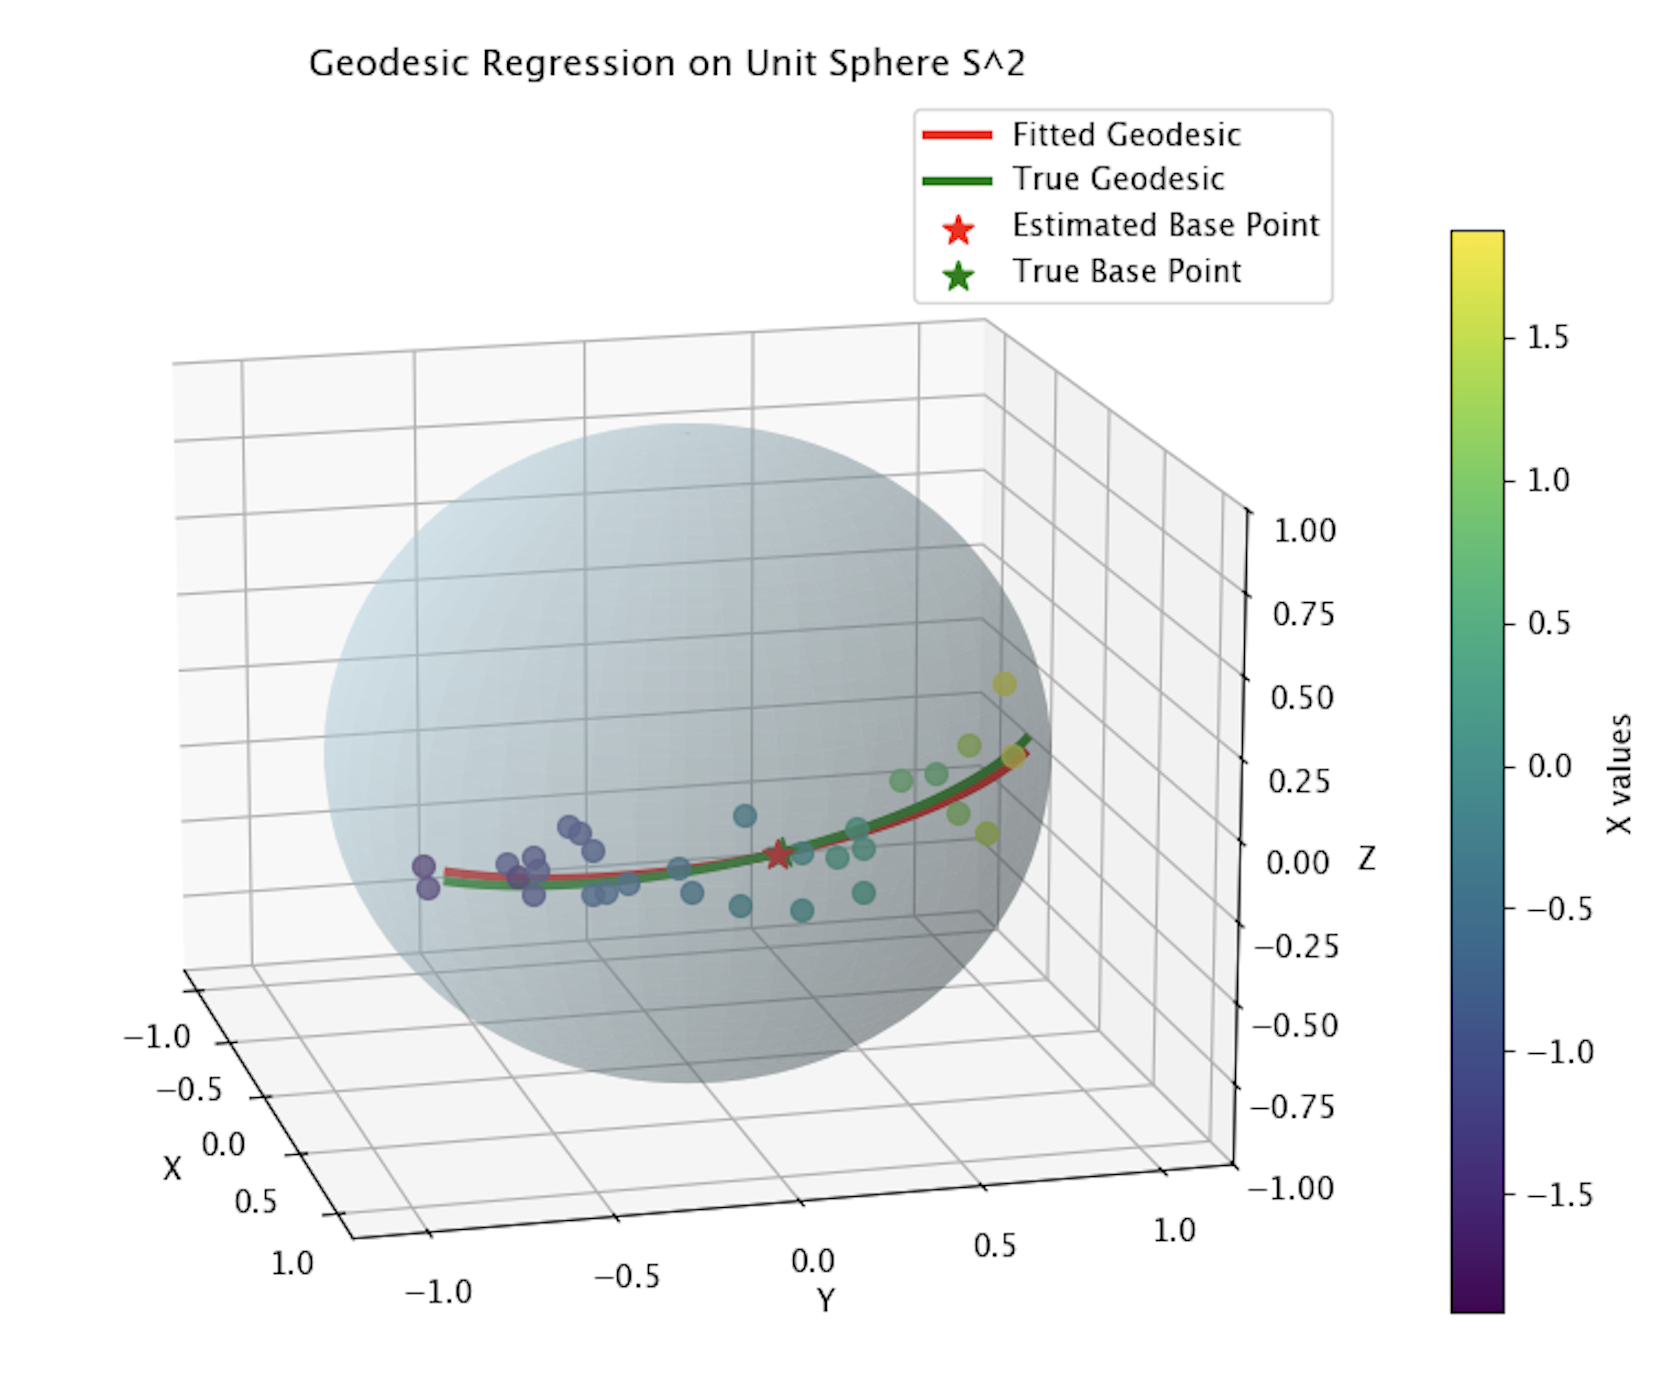
\includegraphics[scale=0.4]{img/geodesic_sphere.png}
      \caption{} 
    \end{figure}
  \end{example}

\subsection{Multiple Geodesic Regression} 

  Note that this was a model for a path in some manifold, and naturally we would like to extend this to have multiple covariates. Kim in 2014 did exactly that, and provided a framework for multivariate general linear models in \cite{2014kim}. 

\subsection{Robust Geodesic Regression}

\section{Frechet Regression}


\bibliography{./bibfile}
\bibliographystyle{alpha}
\end{document}
